
\documentclass[12pt,epsfig,color,russian]{article}
\usepackage[russian]{babel}
\usepackage{epsfig}
\usepackage{color}

\topmargin=0cm
\hoffset -30mm
\voffset -12mm
\setlength{\unitlength}{1mm}
\parindent=10mm
\textheight=250mm
\textwidth=185mm
\pagestyle{empty}

\begin{document}
\sf\Large
\centerline{\underline{\Huge\bf Классическая механика}}
\centerline{кинематика + динамика}
{\sl Г.Галилей (1564-1642)      И.Ньютон (1642-1727)       Л.Эйлер (1707-1783)}

хорошее приближение к действительности (если речь не идет о больших скоростях, больших или малых объектах).

\begin{itemize}
\item Пространство
\item Время
\item Тело
\item Материальная точка
\item Движение
%\item Система координат
\end{itemize}


\centerline{\underline{\Huge\bf КИНЕМАТИКА}}

\underline{Прямолинейное равномерное движение}\\

Движение вдоль прямой; равные $\Delta S$ за равные $\Delta t$.

 \setlength{\unitlength}{1mm}
  \begin{picture}(180,110)(0,0)
  %\put(0,0){\framebox(180,110)[b]{}}
   \put(0,-3){\includegraphics{GP002F01.eps}}
 \put( 170, 96){\makebox(0,0)[tr]{\parbox{85mm}
     {
     \begin{flushright}
      Пройденный путь: $S=f(t)$\\
      $S_x=f_1(t)$\\
      $S_y=f_2(t)$\\
      $S_z=f_3(t)$
     \end{flushright}
         }}}
  \end{picture}\\[3mm]
\newpage

{\bf\underline{Скорость равномерного движения} - физ. величина,
прямо пропорциональная пройденному пути
и обратно пропорцио\-нальная затраченному времени.}

\begin{displaymath}
v = \frac{\Delta S}{\Delta t}\;\;\;{\color{blue}(= const)}
\end{displaymath}
 \\[1mm]
 \setlength{\unitlength}{1mm}
  \begin{picture}(180,100)(0,0)
  %\put(0,0){\framebox(180,110)[b]{}}
   \put(20,-3){\includegraphics{GP002F02.eps}}
  \end{picture}\\[3mm]

{\bf\underline{\color{red}Неавномерное движение:}}
\begin{enumerate}
\item {\underline{\bf OA}} -- торможение
\item {\underline{\bf AB}} -- остановка (состояние покоя)
\item {\underline{\bf BC}} -- ускорение
\item {\underline{\bf CD}} -- равномерное движение
\end{enumerate}

{\bf\underline{Средняя скорость:}}\hspace{10mm}
%\begin{displaymath}
$   v_{mean} =  \langle v\rangle  = \overline{v} =  \frac St$\\
%\end{displaymath}

{\bf\underline{Мгновенная скорость в момент $t=\tau$ :}}

\begin{displaymath}
   v(\tau) = \lim_{\Delta t\rightarrow0}\frac{S(\tau+\Delta t)-S(\tau)}{\Delta t} = \frac{dS}{dt}(\tau)= \dot{S}(\tau)
\end{displaymath}
\newpage

 \setlength{\unitlength}{1mm}
  \begin{picture}(180,110)(0,0)
  %\put(0,0){\framebox(180,110)[b]{}}
   \put(0,-3){\includegraphics{GP002F03.eps}}
  \end{picture}\\[3mm]

\Large\sf Путь, пройденный за время от $t_1$ до $t_2$ -- ?
\begin{displaymath}
S = \sum_i \overline{v_i}\cdot \Delta t_i = \int_{t_1}^{t_2}v(t)dt
\end{displaymath}
 \\[1mm]

\underline{\bf Равнопеременное прямолинейное движение}\\[2mm]

Ускорение (положительное или отрицательное):
\begin{displaymath}
v = v_0 + a\cdot t\;\;\;\;\;\;\;\;\;\;\;a = \frac{\Delta v}{\Delta t}
\end{displaymath}

Более точно:
\begin{displaymath}
a = \lim_{\Delta t\rightarrow 0}\left(\frac{\Delta v}{\Delta t}\right)=\frac{dv}{dt}=\dot{v}=\ddot{s}= const
\end{displaymath}

Путь:
\begin{displaymath}
S = \int_{t_1}^{t_2}v(t)dt = v_0\cdot (t_2-t_1) + \frac{a\cdot \left(t_2-t_1\right)^2}2
\end{displaymath}
\newpage
\underline{\bf Произвольное прямолинейное движение}\\[2mm]

Если задан закон, по которому происходит движение
\begin{displaymath}
 S= f(t)\;\;\;,
\end{displaymath}

то мы всегда сможем найти скорость, ускорение и путь:
\begin{displaymath}
v = \dot{s} = \frac{df}{dt}
\end{displaymath}
\begin{displaymath}
a = \dot{v} = \ddot{s} = \frac{d^2f}{dt^2}
\end{displaymath}
\begin{displaymath}
s = s_2 - s_1 = f(t_2) - f(t_1) \rule[-7mm]{0mm}{12mm}
\end{displaymath}

Поскольку движение имеет {\bf направление}, то s, v и a -- векторы (обозначаются как {\bf s}, {\bf v}, {\bf a} или $\vec{s}$, $\vec{v}$, $\vec{a}$). Все сказанное справедливо (в векторном виде) для криволинейного движения. Положение в пространстве -- радиус-вектор $\vec{r}$.\\
 \setlength{\unitlength}{1mm}
  \begin{picture}(180,110)(0,0)
  %\put(0,0){\framebox(180,110)[b]{}}
   \put(15,-3){\includegraphics{GP002F04.eps}}
  \end{picture}\\[3mm]


\newpage
 \setlength{\unitlength}{1mm}
  \begin{picture}(180,45)(0,0)
  %\put(0,0){\framebox(180,65)[b]{}}
   \put(15,-3){\includegraphics{GP002F05.eps}}
  \end{picture}\\[1mm]

Составляющие ускорения -- тангенциальное и нормальное (радиальное, центростремительное):
 $ \;\;\;\;\vec{a}\;=\;\vec{a_t}\;+\;\vec{a_n}$

 \setlength{\unitlength}{1mm}
  \begin{picture}(180,80)(0,0)
  %\put(0,0){\framebox(180,70)[b]{}}
   \put(15,-3){\includegraphics{GP002F06.eps}}
  \end{picture}\\[1mm]

 \begin{displaymath}
  |dV_t| = |V_2|-|V_1|\;;\;\;\;\;\;  |dV_n| = |V_1|\cdot \varphi
 \end{displaymath}

 \begin{displaymath}
  |a_t| = \lim_{dt\rightarrow0}\frac{|dV_t|}{dt};\;\;\;\;\; \vec{a_t}\parallel\vec{V}
 \end{displaymath}

 \begin{displaymath}
  |a_n| = \lim_{dt\rightarrow0}\frac{|dV_n|}{dt} = \lim_{dt\rightarrow0}\frac{|V_1|\cdot\varphi}{dt}=
  \lim_{dt\rightarrow0}\left(|V_1|\cdot\frac{\varphi}{AB}\cdot\frac{AB}{dt}\right)=
  \frac{|V|^2}R
 \end{displaymath}

 \begin{displaymath}
  \vec{a_n}\parallel \vec{R}\perp \vec{V}
 \end{displaymath}

  \underline{Равномерное} движение по кривой: $\;\;\;|V|$=const, $\;\;\;\; \vec{a}=\vec{a_n}\perp\vec{V}$.
\newpage

  \underline{\bf Кинематика (абсолютно) твердого тела}\\

  {\bf Поступательное движение --} все точки тела имеют одинаковые скорости и ускорения:

 \setlength{\unitlength}{1mm}
  \begin{picture}(180,65)(0,0)
  %\put(0,0){\framebox(180,80)[b]{}}
   \put(15,0){\includegraphics{GP002F07.eps}}
  \end{picture}\\[1mm]

  {\bf Вращение --} все точки тела описывают окружности с центрами на {\sl оси вращения}:

 \setlength{\unitlength}{1mm}
  \begin{picture}(180,92)(0,0)
  %\put(0,0){\framebox(180,100)[b]{}}
   \put(0,0){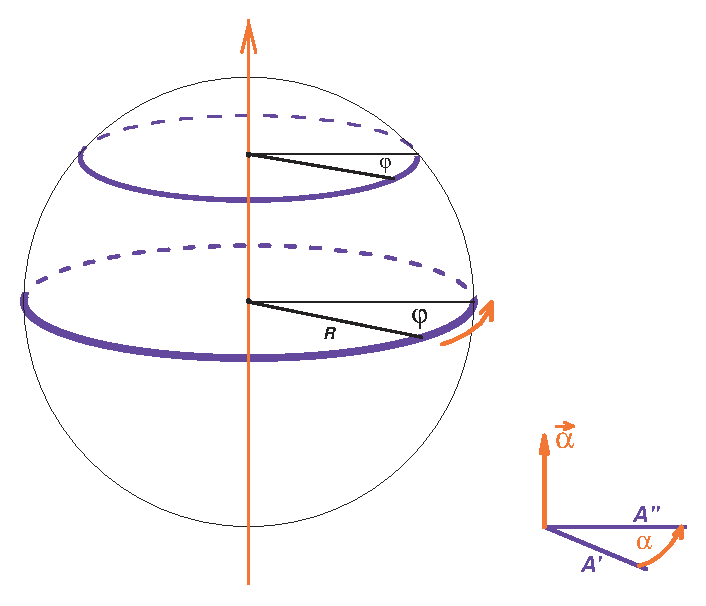
\includegraphics{GP002F08.eps}}
 \put( 180, 92){\makebox(0,0)[tr]{\parbox{85mm}
     {
     \centerline{\underline{Угловая скорость:}}
      \begin{displaymath}
      \omega=\dot{\varphi}=\frac{d\varphi}{dt}
      \end{displaymath}
     \centerline{\underline{Угловое ускорение:}}
      \begin{displaymath}
      \beta=\dot{\omega}=\ddot{\varphi}=\frac{d\omega}{dt}=\frac{d^2\varphi}{dt^2}
      \end{displaymath}
     }}}
 \put( 175, 0){\makebox(0,0)[br]{\parbox{50mm}
     {
      \centerline{Угол как вектор:}
      \begin{displaymath}
      \vec{\alpha}=\alpha\cdot\frac
          {\left[\vec{A'}\times\vec{A''}\right]}
          {\left|\left[\vec{A'}\times\vec{A''}\right]\right|}
      \end{displaymath}
     }}}
  \end{picture}\\

Связь линейной и угловой скорости:

      \begin{displaymath}
      V=\lim_{\Delta t\rightarrow0}\frac{\Delta S}{\Delta t}=\frac{d(R\cdot\varphi)}{dt}=
      \omega R;\;\;\;\;\;\;\;\vec{V}=\left[\vec{\omega}\times\vec{R}\right]
      \end{displaymath}
\newpage

\underline{\bf Линейные и аксиальные векторы}\\

Линейные (истинные) векторы -- те, что связаны с поступательным движением или направлением в пространстве:

 \begin{displaymath}
 \vec{X}, \vec{Y}, \vec{Z}, \vec{V}, \vec{R}, \vec{a}, \vec{F},
 \end{displaymath}

Аксиальные векторы -- те, что связаны с вращением:

 \begin{displaymath}
 \vec{\varphi}, \vec{\alpha}, \vec{\beta}, \vec{L}, \vec{M}
 \end{displaymath}

Они отличаются своими свойствами симметрии: при зеркальном отра\-жении (то есть, при замене $X \rightarrow -X$) линейные векторы меняют знак, а аксиальные - не меняют.

 \setlength{\unitlength}{1mm}
  \begin{picture}(180,150)(0,0)
  %\put(0,0){\framebox(180,150)[b]{}}
   \put(15,0){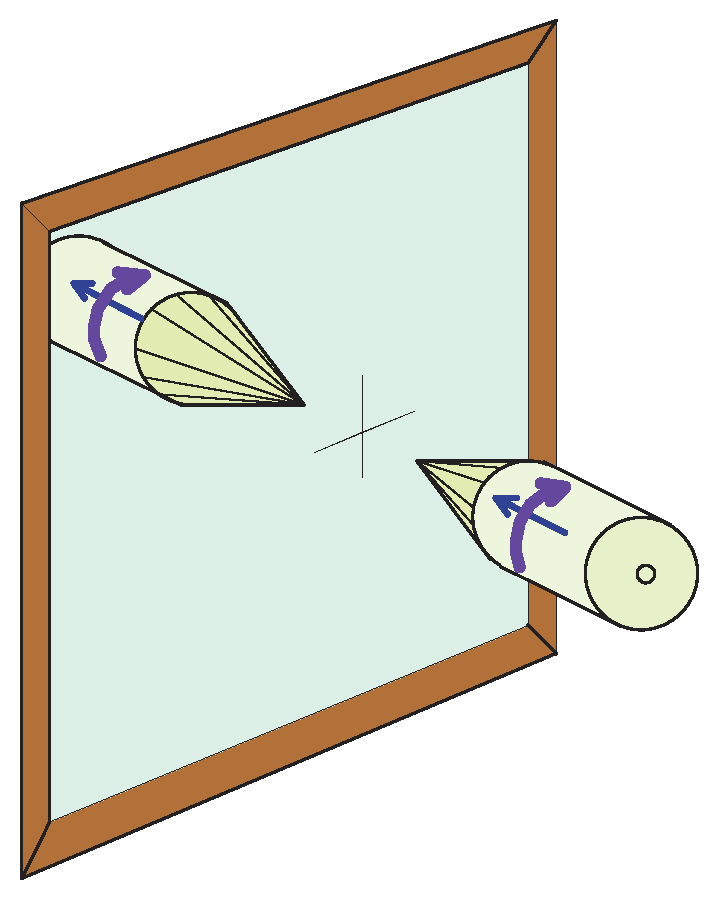
\includegraphics{GP002F09.eps}}
   \put(48, 105){\makebox(0,0)[c]{\color{blue}\Huge\bf $\vec{\omega}_2$}}
   \put(48, 70){\makebox(0,0)[c]{\color{red}\Huge\bf $\vec{V}_2$}}
   \put(120, 70){\makebox(0,0)[c]{\color{blue}\Huge\bf $\vec{\omega}_1$}}
   \put(120, 35){\makebox(0,0)[c]{\color{red}\Huge\bf $\vec{V}_1$}}
   \put(150,110){\makebox(0,0)[c]{\color{red}\Huge\bf $\vec{V}_2 = -\vec{V}_1$}}
   \put(150, 90){\makebox(0,0)[c]{\color{blue}\Huge\bf $\vec{\omega}_2 = +\vec{\omega}_1$}}
  \end{picture}\\[1mm]
\newpage
\begin{flushright}
{\color{green}\LARGE\sl ШПАРГАЛКА}
\end{flushright}

\underline{\bf Связь декартовых и сферических координат}

 \begin{displaymath}
 \left\{\vec{x}, \vec{y}, \vec{z}\right\}
 \;\;\;\leftrightarrow \;\;\;
 \left\{\vec{r}, \vec{\theta}, \vec{\varphi}\right\}
 \end{displaymath}

 \setlength{\unitlength}{1mm}
  \begin{picture}(180,130)(0,0)
  %\put(0,0){\framebox(180,130)[b]{}}
   \put(25,0){\includegraphics{GP002F10.eps}}
  \end{picture}\\[1mm]
 \begin{displaymath}
 \begin{array}{ccccc}
 0&\leq&r&&\\
 0&\leq&\theta&\leq&\pi\\
 0&\leq&\varphi&\leq&2\pi
 \end{array}
 \end{displaymath}

 \begin{displaymath}
 \left\{
 \begin{array}{ccl}
 x&=&r\sin\theta\cos\varphi\\
 y&=&r\sin\theta\sin\varphi\\
 z&=&r\cos\theta
 \end{array}
 \right\}\;\;\;
 \leftrightarrow\;\;\;
 \left\{
 \begin{array}{ccl}
 r&=&\sqrt{x^2+y^2+z^2}\\
 \theta&=&\arccos\left(z/r\right)\\
 \varphi&=&\arctan\left(y/x\right)
 \end{array}
 \right\}
 \end{displaymath}

 \begin{displaymath}
dx\cdot dy\cdot dz\;\;=\;\;dV\;\;=\;\;r^2\cdot dr\cdot\sin\theta\cdot d\theta\cdot d\varphi
 \end{displaymath}


\newpage
\begin{flushright}
{\color{green}\LARGE\sl ШПАРГАЛКА}
\end{flushright}
\centerline{\huge\underline{Правила векторной алгебры}}
\begin{itemize}
\item длина вектора (модуль):
 \begin{displaymath}
 |\vec{A}| = \sqrt{A_x^2+A_y^2+A_z^2}
 \end{displaymath}
\item сложение (вычитание):
 \begin{displaymath}
 \vec{C} = \vec{A} \pm \vec{B}\;\;\;\Leftrightarrow\;\;\;
 \left\{\begin{array}{cc}C_x &= A_x\pm B_x\\
                         C_y &= A_y\pm B_y\\
                         C_z &= A_z\pm B_z\end{array}\right.
 \end{displaymath}
\item умножение на число (масштабирование):
 \begin{displaymath}
 \vec{C} = k\cdot\vec{A} \;\;\;\Leftrightarrow\;\;\;
 \left\{\begin{array}{cc}C_x &= k\cdot A_x\\
                         C_y &= k\cdot A_y\\
                         C_z &= k\cdot A_z\end{array}\right.
 \end{displaymath}
\item дифференцирование:
 \begin{displaymath}
 \vec{C} = \frac{\vec{dA}}{dt} \;\;\;\Leftrightarrow\;\;\;
 \left\{\begin{array}{cc}C_x &= {dA_x}/{dt}\\
                         C_y &= {dA_y}/{dt}\\
                         C_z &= {dA_z}/{dt}\end{array}\right.
 \end{displaymath}
\item скалярное перемножение двух векторов:
 \begin{displaymath}
 C = \left(\vec{A},\vec{B}\right) = \vec{A}\cdot\vec{B}\;\;\;\Leftrightarrow\;\;\;
 C = A_x\cdot B_x + A_y\cdot B_y + A_z\cdot B_z =|A|\cdot|B|\cdot \cos\theta
\end{displaymath}
\item векторное перемножение двух векторов:
 \begin{displaymath}
 \vec{C} = \left[\vec{A},\vec{B}\right] = \vec{A}\times\vec{B}\;\;\;\Leftrightarrow\;\;\;
 \left\{\begin{array}{cc}C_x &= A_y\cdot B_z - A_z\cdot B_y\\
                         C_y &= A_z\cdot B_x - A_x\cdot B_z\\
                         C_z &= A_x\cdot B_y - A_y\cdot B_z\end{array}\right.
 \end{displaymath}
 \begin{displaymath}
  |C|=|A|\cdot|B|\cdot\sin\theta;\;\;\;\; \vec{C}\perp\vec{A};\;\;\;\vec{C}\perp\vec{B}
\end{displaymath}
\end{itemize}

\end{document}
\newpage


\centerline{\underline{\Huge\bf ДИНАМИКА}}

\centerline{\sl изучает взаимодействие тел, приводящее к изменению их движения}
\vspace{2mm}
\underline{\bf Первый закон Ньютона (принцип инерции)}
\begin{center}
\fbox{\parbox{180mm}{\color{blue}\bf Всякое тело сохраняет состояние покоя или равномерного и прямолинейного движения, пока
воздействие со стороны других тел не заставит его изменить это состояние.}}\\[1mm]
(Здесь тело -- как материальная точка, то есть, вращение исключается.)
\end{center}

Наблюдения: 1зН справедлив не для каждой системы отсчета.

\fbox{Инерциальная система} -- та, по отношению к которой 1зН выполняется.

Гелиоцентрическая система. Всякая система, движущаяся относительно нее равномерно и прямолинейно.
\fbox{\color{blue}Инерциальные системы существуют.}\\

\underline{\bf Второй закон Ньютона}
\begin{center}
\fbox{\parbox{180mm}{\color{blue}\bf Изменение движения пропорционально приложенной силе и происходит в том направлении, в каком действует сила.}}\\[1mm]
\end{center}
Физ. величина СИЛА характеризует воздействие одних тел на другие, в результате которого тела приобретают ускорение.
\begin{displaymath}
 f=k\cdot a\;\;\;\;\;\;\;\;\vec{f}=k\cdot\vec{a}
 \end{displaymath}
Более удобное измерение силы: пружинный динамометр\\
 \setlength{\unitlength}{1mm}
  \begin{picture}(180,40)(0,0)
   %\put(0,0){\framebox(180,40)[b]{}}
   \put(15,0){\includegraphics{L1F17.eps}}
  \end{picture}\\[1mm]
Опыт: {\bf разные} тела от {\bf одинаковой} силы получают {\bf разные} ускорения. Это свойство тел -- физ. величина ИНЕРЦИОННАЯ МАССА.\\
Ньютон: МАССА - это мера количества материи в теле {\sl (не совсем верно)}. МАССА - это именно мера инерции.\\
М.В.Ломоносов: масса изолированной системы = const.
\begin{displaymath}
 \vec{a}=k\cdot\vec{f}/m
 \end{displaymath}
\newpage
Упругие силы, силы тяготения. \underline{\bf Силы трения} -- молекулярное взаимо\-действие между соприкасающимися телами. Трение внешнее (между телом и другими телами; трение покоя) и внутреннее (движение жидкостей и газов).

Сила трения всегда направлена противоположно скорости. Чтобы тело двигалось без ускорения, надо, чтобы внешняя сила уравновешивала силу трения.

 \setlength{\unitlength}{1mm}
  \begin{picture}(180,35)(0,0)
   %\put(0,0){\framebox(180,40)[b]{}}
   \put(10,0){\includegraphics{L1F18.eps}}
  \end{picture}\\[1mm]

Парашютист: 60 м/с (открытие парашюта) => 5-6 м/с.

Сила трения скольжения приблизительно пропорциональна сжи\-мающей силе $F_n$:
\begin{displaymath}
 F_{TP}\simeq\chi\cdot F_n
 \end{displaymath}

 \setlength{\unitlength}{1mm}
  \begin{picture}(180,55)(0,0)
   %\put(0,0){\framebox(180,40)[b]{}}
   \put(45,0){\includegraphics{L1F19.eps}}
   \put(0,50){\makebox(0,0)[tl]{\parbox{60mm}{коэффициент трения $\chi$ зависит от состояния поверхностей и от скорости скольжения}}}
  \end{picture}\\[1mm]

 \setlength{\unitlength}{1mm}
  \begin{picture}(180,55)(0,0)
   %\put(0,0){\framebox(180,40)[b]{}}
   \put(5,0){\includegraphics{L1F20.eps}}
   \put(80,40){\makebox(0,0)[c]{\parbox{85mm}{При V=0 сила трения может быть от 0 до некоего максимума $f$, а при начале движения снижается}}}
   \put(178,30){\makebox(0,0)[tr]{\bf авто: ABS}}
  \end{picture}
\newpage
Рассмотрим движение под действием постоянной силы $\vec{f}$ за время $\Delta t$. Используя 2зН, получим:
\begin{displaymath}
  k\cdot\frac{\vec{f}}{m}=\vec{a}=\frac{\vec{v_2}-\vec{v_1}}{\Delta t}
\end{displaymath}
или, домножив на $m$ и $\Delta t$ :
\begin{displaymath}
 m\vec{v_2}-m\vec{v_1} = k\cdot\vec{f}  \Delta t
\end{displaymath}
Величина $m\vec{v}$ имеет большой физический смысл и называется КОЛИЧЕСТ\-ВО ДВИЖЕНИЯ или ИМПУЛЬС (обозначается как $\vec{p}$ -- от англ. {\sl pulse}).
\begin{displaymath}
\vec{p}\equiv m\vec{v}\hspace{40mm} \frac{\vec{dp}}{dt} = k\cdot\vec{f}
\end{displaymath}

Еще одно определение СИЛЫ: Сила -- векторная величина, пропорцио\-нальная вызываемому ею изменению импульса в единицу времени.

Величина $\vec{f}\Delta t$ тоже имеет персональное название -- ИМПУЛЬС СИЛЫ.

Если положить коэф-т $k$ равным 1, то можно установить единицы измерения для $f$.
\begin{itemize}
\item CGS: $[m]$= г, $\;\;[a]$= см/с$^2\;\;\;\;\Rightarrow\;\;\;[f]$= ДИНА = г$\cdot$см/с$^2$
\item SI: $\;\;\;[m]$= кг, $\;[a]$= м/с$^2\;\;\;\;\Rightarrow\;\;\;[f]$= НЬЮТОН = кг$\cdot$м/с$^2 = 10^5$дин
\end{itemize}
\vspace{2mm}

\underline{\bf Механический принцип относительности (Галилей)}

1зН -- частный случай 2зН при $f=0$.

Движение тела относительно двух различных ниерциальных систем отличается лишь на постоянную разность скоростей, а ускорения -- одина\-ковы. $\Rightarrow$ и силы (по 2зН) одинаковы!\\[3mm]
\fbox{\parbox{185mm}{\color{blue}\bf Никакими механическими опытами, производимыми внутри системы, нельзя решить -- находится ли инерциальная система в состоянии покоя или она равномерно и прямолинейно движется. \color{black}\sl Галилей, 1632 г.  }}\\[1mm]

Принцип относительности Эйнштейна: ({\color{blue}механическими})$\rightarrow$({\color{red}любыми: меха\-ническими, электрическими, оптическими, etc.})
\newpage

\underline{\bf Третий закон Ньютона} {(\sl Как аукнется, так и откликнется)}

\begin{center}
\fbox{\parbox{180mm}{\color{blue}\bf Если тело {\bf B} воздействует на тело {\bf A} с силой $\vec{f_1}$, то и тело {\bf A}, в свою очередь, воздействует на тело {\bf B} с силой $\vec{f_2}$, причем $\vec{f_1}=-\vec{f_2}$.}}
\end{center}
%\\[1mm]

 \setlength{\unitlength}{1mm}
  \begin{picture}(180,65)(0,0)
   %\put(0,0){\framebox(180,65)[b]{}}
   \put(0,0){\includegraphics{L1F21.eps}}
  \end{picture}\\[1mm]

Итак, если взаимодействуют 2 тела A и B ;) с массами $m_1$ и $m_2$, то оба приобретают противоположные ускорения:
\begin{displaymath}
\vec{a_1}=\frac{f_1}{m_1},\;\;\;\;\;\;\vec{a_2}=\frac{f_2}{m_2}
\end{displaymath}

Из 3зН следует, что $\vec{f_1}=-\vec{f_2}$, и поэтому
\begin{displaymath}
\vec{a_1}=-\frac{m_2}{m_1}\cdot\vec{a_2}
\end{displaymath}

Изменение количества движения тел A и B:
\begin{displaymath}
\vec{\Delta p_1}=\vec{f_1}\cdot\Delta t\;\;\;\;\;\;\;\vec{\Delta p_2}=
\vec{f_2}\cdot\Delta t=-\vec{\Delta p_1}
\end{displaymath}

\begin{center}
\fbox{\parbox{180mm}{\color{blue}\bf Насколько в результате взаимодействия импульс одного тела увеличился, настолько импульс другого тела уменьшился.}}\\[1mm]
\end{center}

Обобщая на всю систему из N тел, получаем ЗАКОН СОХРАНЕ\-НИЯ КОЛИЧЕСТВА ДВИЖЕНИЯ (ИМПУЛЬСА): $\sum\vec{p} = $const.

\begin{center}
\fbox{\parbox{180mm}{\color{blue}\bf Полный импульс замкнутой системы остается постоянным во все время движения. \color{red}\sl (Не обнаружено нарушений ни в микро-, ни в макро-мире, ни в квантовой, ни в релятивистской механике)}}
\end{center}

\newpage
Поскольку импульс --- это вектор, то закон сохранения выполняется отдельно для каждой его составляющей:

 \setlength{\unitlength}{1mm}
  \begin{picture}(180,50)(0,0)
   %\put(0,0){\framebox(180,65)[b]{}}
   \put(0,0){\includegraphics{L1F22.eps}}
   \put(180,40){\makebox(0,0)[rt]{\parbox{60mm}{\begin{displaymath}
                                            \left\{ \begin{array}{ccc}
                                            p_x&=&R_x+q_x\\
                                            0&=&R_y+q_y\\
                                            0&=&R_z+q_z
                                                    \end{array}
                                            \right.
                                               \end{displaymath}}}}
  \end{picture}\\[1mm]

Для изолированной системы из N тел:

\begin{displaymath}
 \vec{P}=\sum_i^N\vec{p_i}=const\;\;\;\Leftrightarrow\;\;\;
 \left\{ \begin{array}{ccccc}
 P_x&=& \sum_{i=1}^N p_{xi}&=&const\\
 P_y&=& \sum_{i=1}^N p_{yi}&=&const\\
 P_z&=& \sum_{i=1}^N p_{zi}&=&const
 \end{array}
 \right.
\end{displaymath}
\hspace{3mm}

\underline{\bf Силы при криволинейном движении}

 \setlength{\unitlength}{1mm}
  \begin{picture}(180,80)(0,0)
   %\put(0,0){\framebox(180,90)[b]{}}
   \put(0,0){\includegraphics{L1F23.eps}}
  \end{picture}\\

Как и ускорение, сила имеет 2 компонента: \begin{enumerate}
\item тенгенциальная сила ($\vec{f_t}\parallel\vec{v}$ -- разгоняет или тормозит)
\item центростремительная сила ($\vec{f_n}\perp\vec{v}$ -- заставляет менять направление)
\end{enumerate}
\begin{displaymath}
 \vec{f}=\vec{f_t}+\vec{F_n};\;\;\;\;\;\;\;|f|=\sqrt{f_t^2+f_n^2};\;\;\;\;\;\;\;\;
 |f_n|=ma_n=m \frac{v^2}{R}
\end{displaymath}

\newpage
\noindent
Равномерное движение по кривой: $f_t=0$. Вся сила -- центростремительная.\\[4mm]
Равномерное движение по окружности: $R=$const., $v=\omega R$
\begin{displaymath}
 f_n=m \frac{v^2}{R}=m\omega^2R=4\pi^2m\frac{R}{T^2}
\end{displaymath}

\underline{Центростремительная} сила приложена к телу, а равная ей (но противопо\-ложная по направлению) \underline{центробежная} -- к связям
\\
 \setlength{\unitlength}{1mm}
  \begin{picture}(180,60)(0,0)
   %\put(0,0){\framebox(180,65)[b]{}}
   \put(85,0){\includegraphics{L1F24.eps}}
   \put(0,0){\makebox(0,0)[bl]{\parbox{130mm}{
    Неподвижный вагон, кроме нормальной к рельсам силы $f_0$, оказывает на них боковое давление с силой $f_s=P\;{\rm tg}\alpha$. Надо, чтобы при движении центробежная сила ее скомпенсировала:
   \begin{displaymath}
   P\cdot tg\alpha = mg\cdot tg\alpha = \frac{mv^2}{R}\;\;\;\;\Rightarrow\;\;\;
   tg\alpha = \frac{mv^2}{Rg}
   \end{displaymath}}}}
  \end{picture}\\[1mm]

\underline{\bf Ускоренные системы}
\\
 \setlength{\unitlength}{1mm}
  \begin{picture}(180,40)(0,0)
   %\put(0,0){\framebox(180,65)[b]{}}
   \put(0,0){\includegraphics{L1F25.eps}}
   \put(190,0){\makebox(0,0)[br]{\parbox{90mm}{
   В Лаб.системе: вагон ускоряется, шар отстает.\\
   В системе вагона: шар покатился назад с ускорением $-a$, как если бы появилась сила
   $\vec{f}=-m\vec{a}$
   }}}
  \end{picture}\\[1mm]

Фиктивная сила, которую приходится вводить в ускоренной системе отсчета, чтобы в ней выполнялся 2 закон Ньютона -- \underline{инерционная сила} или \underline{сила инерции}.
\\
 \setlength{\unitlength}{1mm}
  \begin{picture}(180,90)(0,0)
   %\put(0,0){\framebox(180,80)[b]{}}
   \put(0,0){\includegraphics{L1F26.eps}}
   \put(190,0){\makebox(0,0)[br]{\parbox{130mm}{
   \begin{enumerate}
   \item{\bf $\vec{a}=0$ (Лифт стоит на месте или движется равномерно.)}
        Гиря давит на весы своим весом $\vec{P}=m\vec{g}$. Весы давят на гирю с такой же силой и уравновешивают ее вес. (В обеих {\bf инерционных} системах координат)
   \item{\bf $\vec{a}>0$ (Лифт ускоряется вверх.)}
    \begin{itemize}
    \item В Лаб.системе: Чтобы гиря тоже начала ускоряться вместе с лифтом, весы давят на нее снизу с дополнительной силой $\vec{f\prime}=m\vec{a}$. По 3зН гиря давит на весы с такой же силой.
    \item В системе лифта: появилась сила инерции $\vec{f\prime\prime}=-m\vec{a}$, которая добавилась к весу гири.
    \end{itemize}
   \end{enumerate}
   }}}
  \end{picture}\\[1mm]
  ОТО Эйнштейна: Вселенная относительно системы лифта дернулась вниз с ускорением $-\vec{a}$ и создала дополнительное гравитационное поле, направ\-ленное туда же:
   $g\;\;\;\rightarrow\;\;\;g\prime=(g+a)$.\\[1mm]

\underline{\bf Вращающиеся системы}
\\
 \setlength{\unitlength}{1mm}
  \begin{picture}(180,100)(0,0)
   %\put(0,0){\framebox(180,65)[b]{}}
   \put(0,0){\includegraphics{L1F27.eps}}
   \put(190,0){\makebox(0,0)[br]{\parbox{100mm}{
   В инерционной гелиоцентрической системе: чтобы тело А на широте $\varphi$ вращалось вместе с Землей вокруг ее оси, надо, чтобы часть его веса $P_0$ играла роль центростремительной силы ${\color{green}f}=m\omega^2r=m\omega^2R\cos\varphi$.\\
   В системе, связанной с Землей: 1) направленный к центру Земли вес $P_0$  и 2) {\sl инерционная центробежная сила} ${\color{red}f\prime}=m\omega^2r$, направленная от оси. Их сумма - кажущийся вес ${\color{magenta}P}$.\\
   Масштаб: $f/P_0=\omega^2R\cos\varphi/g\simeq\cos\varphi/289$
   }}}
  \end{picture}\\[1mm]
На экваторе ($\varphi=0$): $f/P_0$ -- максимально; \hfill{} $f_{\max}/P_0=\omega^2R/g=v^2/gR$\\
Обращается в 1 при $v=\sqrt{gR}\simeq7.9$ км/с
\newpage
\centerline{\underline{\bf Сила Кориолиса}}
 \setlength{\unitlength}{1mm}
  \begin{picture}(180,240)(0,0)
   %\put(-5,-10){\framebox(180,240)[b]{}}
   \put(0,-10){\includegraphics{L1F28.eps}}
   \put(190,0){\makebox(0,0)[br]{\parbox{100mm}{la-la-la
   }}}
  \end{picture}\\[1mm]

\end{document} 